

\documentclass[10pt]{sensys-proc}
\usepackage{graphicx}
\usepackage{balance}
\usepackage{comment}
\newcommand{\redcolor}[1]{\textcolor{red}{#1}}

\newcommand{\figref}[1]{Figure~\ref{#1}}
\newcommand{\secref}[1]{Section~\ref{#1}}
\newcommand{\tabref}[1]{Table~\ref{#1}}
\newcommand{\algoref}[1]{Algorithm~\ref{#1}}
\usepackage{graphicx}
\usepackage{subfig}
\usepackage{blindtext}
\usepackage{array}
\usepackage{caption}
\usepackage{url}
\usepackage{epstopdf}
\usepackage{multirow}
\usepackage{xcolor,colortbl}

\newcommand{\pushline}{\Indp}
\definecolor{Gray}{gray}{0.91}
\newcolumntype{a}{>{\columncolor{Gray}}c}

\numberofauthors{2}

\author{
%
% The command \alignauthor (no curly braces needed) should
% precede each author name, affiliation/snail-mail address and
% e-mail address. Additionally, tag each line of
% affiliation/address with \affaddr, and tag the
%% e-mail address with \email.
\alignauthor Alice Security \\
        \affaddr{Department of Computer Science}\\
        \affaddr{University of Southern California}\\
       \email{alice@example.edu}
\alignauthor Bob Privacy \\
    \affaddr{Networked Embedded Systems Group}\\
    \affaddr{Swedish Institute of Computer Science}\\
    \email{bob@example.se}
}

\title{Its Different: Hitchiker’s Tryst with Energy Consumption Patterns in India}

\crdata{978-1-4503-1169-4}
\conferenceinfo{SenSys'13,} {November 11--15, 2013, Rome, Italy.}
\CopyrightYear{2013}

\begin{document}

\maketitle

\begin{abstract}
This paper provides a sample of a \LaTeX\ document for ACM Sensys. 
It complements the document \textit{Author's (Alternate) Guide to
Preparing ACM SIG Proceedings Using \LaTeX$2_\epsilon$\ and Bib\TeX}.
This source file has been written with the intention of being
compiled under \LaTeX$2_\epsilon$\ and BibTeX.

To make best use of this sample document, run it through \texttt{pdflatex}
and \texttt{bibtex} to directly produce a pdf document.
\end{abstract}

% A category with the (minimum) three required fields
\category{H.4}{Information Systems Applications}{Miscellaneous}
%A category including the fourth, optional field follows...
\category{D.2.8}{Software Engineering}{Metrics}[complexity measures, performance measures]

\terms{Delphi theory}

\keywords{ACM proceedings, \LaTeX, text tagging}

\section{Introduction+Related Work}
  \label{sec:intro}

\begin{itemize}
\item Why buildings must be targeted for energy \cite{evans09}
\item Importance of feedback \cite{darby}
\item Why we need deployments
\item Deployments- Residential, Office \cite{yuvraj_ipsn, batra}
\item Previous such residential deployments, some of which were presented in Buildsys itself \cite{hitchhiker_residential,hitchhiker_wsn,scale_wsn}
\item Some applications-NILM\cite{hart,survey1}, Fixture Finder \cite{fixturefinder}
\item Specific learnings from our deployment, some of them complement the ones given earlier \cite{hitchhiker_residential}
\begin{itemize}
\item Glowing LED in night 
\item Deployments should be transparent
\item Noisy server owing to dust (specific to developing countries)
\item Electricity failure- as a consequence all systems should be capable to restart upon resumption of electricity
\item Unreliable internet -Forcing to use Sense-Store-Upload paradigm
\item Normalization -Voltage fluctuation, different measurement by different instruments


\end{itemize}
\end{itemize}
Also deployment was maintained as an open source project. Shows how we faced issues and tackled them. Also contains metadata log provided by the end user.

\section{Deployment Overview}
Over the past year, we have deployed sensors across 22 homes. While 20 of these homes have been instrumented only with smart electricity meters, 2 homes have been extensively instrumented with upto 32 sensors measuring electricity, water and ambient parameter. \figref{fig:overall} shows the deployment in a 3 storey home where 32 sensors, 5 single board computers and 3 routers were used. 
\subsection{Sensing Infrastructure}
For our sensing, we took a ``leave no stone unturned'' approach, where  we chose to monitor as many physical parameters (such as ambient conditions, electricity usage, water usage) and non-physical parameters(such as network strength etc.). However, it must be noted, that we chose to deploy sensors in a way that home users can continue their regular routine without getting affected. We describe the various sensors to monitor electricity, water and ambient conditions below:

\noindent\textbf{Electricity monitoring:} A typical home electricity setup involves a meter which is installed by utility companies and measures overall electricity usage. Further electric cabling is divided into various Miniature Circuit Breakers (MCB's) which control separate circuits. Typical installations involve putting separate MCB's for heavier loads such as air conditioners and clubbing various lights, fans and other smaller loads into separate MCB. Further each individual appliance is controlled via a switch. There are two types of appliances- i) plug loads like refrigerator and electric iron, which need to be physically ``plugged" into the sockets; ii) loads like lights and fans, which do not need to be ``plugged" in by the user. We highlight the above described home electricity distribution in \figref{fig:overall}. We have 3 different resolutions at which electricity can be monitored:
\begin{enumerate}
\item \textbf{Meter level:} We use Schneider Electric EM6400\footnote{\url{To put}} smart meter to instrument the main power supply. While cheaper variants from the same company were available, we chose to use EM6400 since, in addition to real power, it also provides reactive power. This additional information has been known to be useful for NILM applications\cite{hart}. \figref{fig:em6400} shows EM6400 smart meter deployed in the electricity panel.

\item \textbf{Circuit level:} We used our in-house developed Current transformer (CT) based monitoring circuits which can be clamped to individual MCB's. \redcolor{Manoj write 1-2 lines about this circuit}. CT deployment is shown in \figref{fig:ct}.

\item \textbf{Appliance level:} We used jPlug\footnote{A variant of nPlug\cite{nplug}} to measure individual appliance power consumption for 9 plug-load type appliances. We also used Current Cost based CT to measure the power consumption for electric motor (used to pump water), which is not a plug-load, yet has significant power consumption. jPlug and Current Cost CT deployment are shown in \figref{fig:jplug} and \figref{fig:cc} respectively.
\end{enumerate}
More details regarding sensors used for electricity monitoring are provided in \tabref{tab:sensing}.

\noindent \textbf{Water monitoring:} There are few differences in water distribution in India and US. In India, there are separate water lines for drinkable and non-drinkable water. Also, overhead water tanks (typically 1000 liters capacity) are used to store water. Electric motors are used to push water against gravity to be stored in the tank. Thus, the flow can be summarized as follows: 1) Water from utility comes to the home; 2) Electric motor is used to pump the water up to the tank; 3) Water flows downward from the tank when ever water is consumed. Thus, we put a water meter at the inlet (coming from the utility) and the outlet from the water tank (flowing downwards). 


\noindent Digital water meters are very expensive. Thus, we chose to use in-line water meters, which measure water volume flowing through them. These water meters have a 400 ma current loop \redcolor{Manoj: Add details} and send a pulse every few liters. The precision is based on the quality of the sensor and the diameter of the water pipe. The water meter we used for overhead tank gives a pulse every 10 liters, whereas the one used for inlet supply from utility gives a pulse every 1 liter. These pulses can be measured using the circuit diagram for 400 ma loop shown in ... \figref{fig:water_meter} shows the water meter deployed inline at the overhead tank.

\noindent \textbf{Ambient conditions monitoring:} 




\begin{table*}
\caption{Deployment}

\label{tab:sensing}
\tabcolsep=0.015cm
\begin{tabular}{|l|l|l|l|l|l|l|}
\hline
Sensor&Sensor&Sampling&Resolution&Qua-&Commu-&Observed\\
name&type&frequency&&ntity&nication&parameters\\
&&(Hz)&&&&\\
\hline

EM6400&Electric Meter&1&Home&1&RS 485, WiFi&Voltage, Current,\\ 
&&&&&&Frequency\\ \hline
Analog&Water Meter&5&Main supply and tank&2&\\ \hline
Homeseer HSM-100&Ambient multisensors&1 (for light, temperature)&Room &6&ZWave&Light, temperature\\ 
                &&and polling for PIR&&&& and motion\\ \hline
Android phones&Ambient multisensors& check from funf&Room&5&Manual\\ \hline
Prototype CT&Current Transformers&20&MCB&8&WiFi\\ \hline
jPlug&Appliance electric meter & 1 &Appliance&9&WiFi\\ \hline
Current Cost&Appliance CT&0.1&Appliance&1&Proprietary\\ \hline
\hline

\end{tabular}


\end{table*}

\subsection{Communication and Computation Infrastructure}
Following computation resources (SBC/Servers were used)
\begin{itemize}
\item X RPi
\item Plug Computers
\item Main server
\end{itemize}
Following sensors were used.
\begin{itemize}
\item EM6400 smart meter: We used pyModbus to sample at 1 Hz. Gives 40 parameters including reactive power. Reactive power can greatly help in improving NILM accuracy \cite{hart}. 
\item Appliance level meters: jPlug and Current Cost. jPlug gives data at 1 Hz and gives 10 parameters including reactive power. Current cost was needed for one appliance- electric motor.
\item CT monitoring: Custom hardware based on  XYZ.
\item Multisensors: Measure motion (based on polling), light and temperature
\item Water meter: 10 litre events. 
\item Android phones measuring x, y, z using FunF Journal\footnote{\url{http://www.funf.org/journal.html}}
\end{itemize}
Apart from this following soft-sensor streams were collected.
\begin{itemize}
\item Network statistics
\item CPU, Memory usage for all computing resources. This was to serve as preventive measure.
\item Weather streams
\end{itemize}
\begin{figure}     
    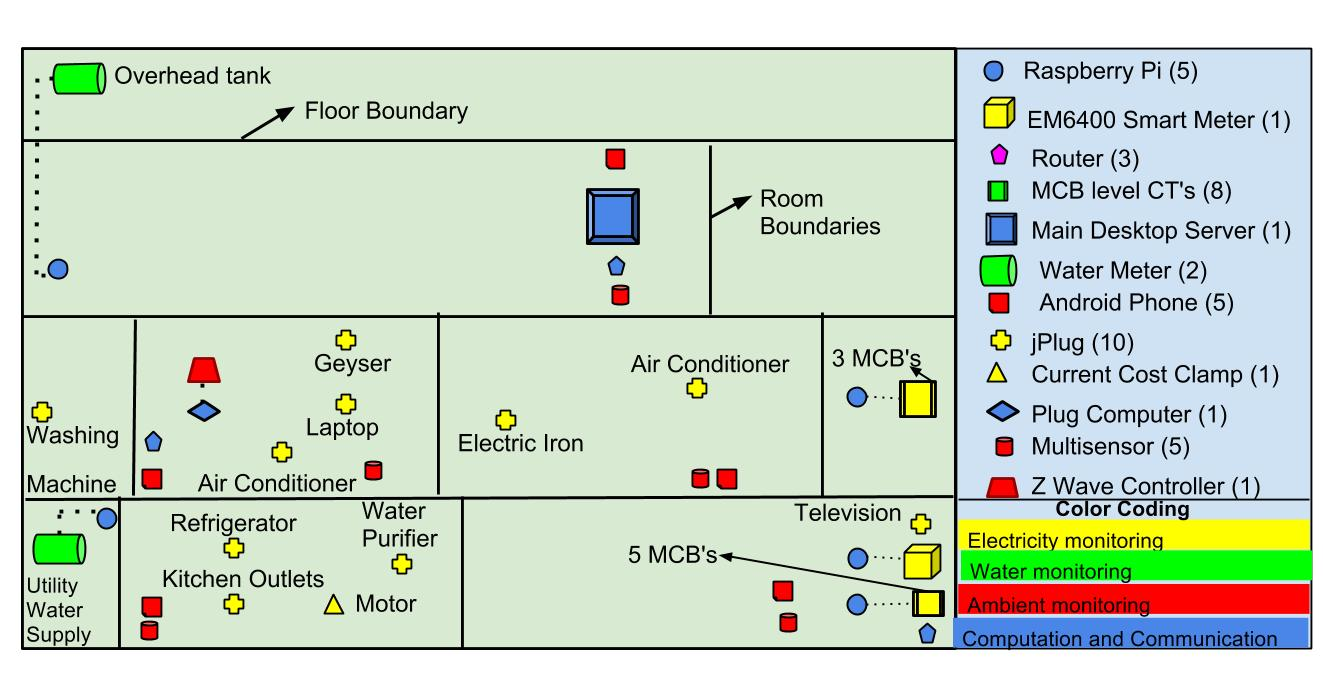
\includegraphics[scale=0.2]{./figures/overall_deployment.jpg}    
    \caption{Schematic showing overall home deployment}   
    \label{fig:overall}
   
\end{figure}


\begin{figure*} 
    
    \subfloat[\scriptsize EM6400 Smart Meter]{
    \label{fig:em6400}
    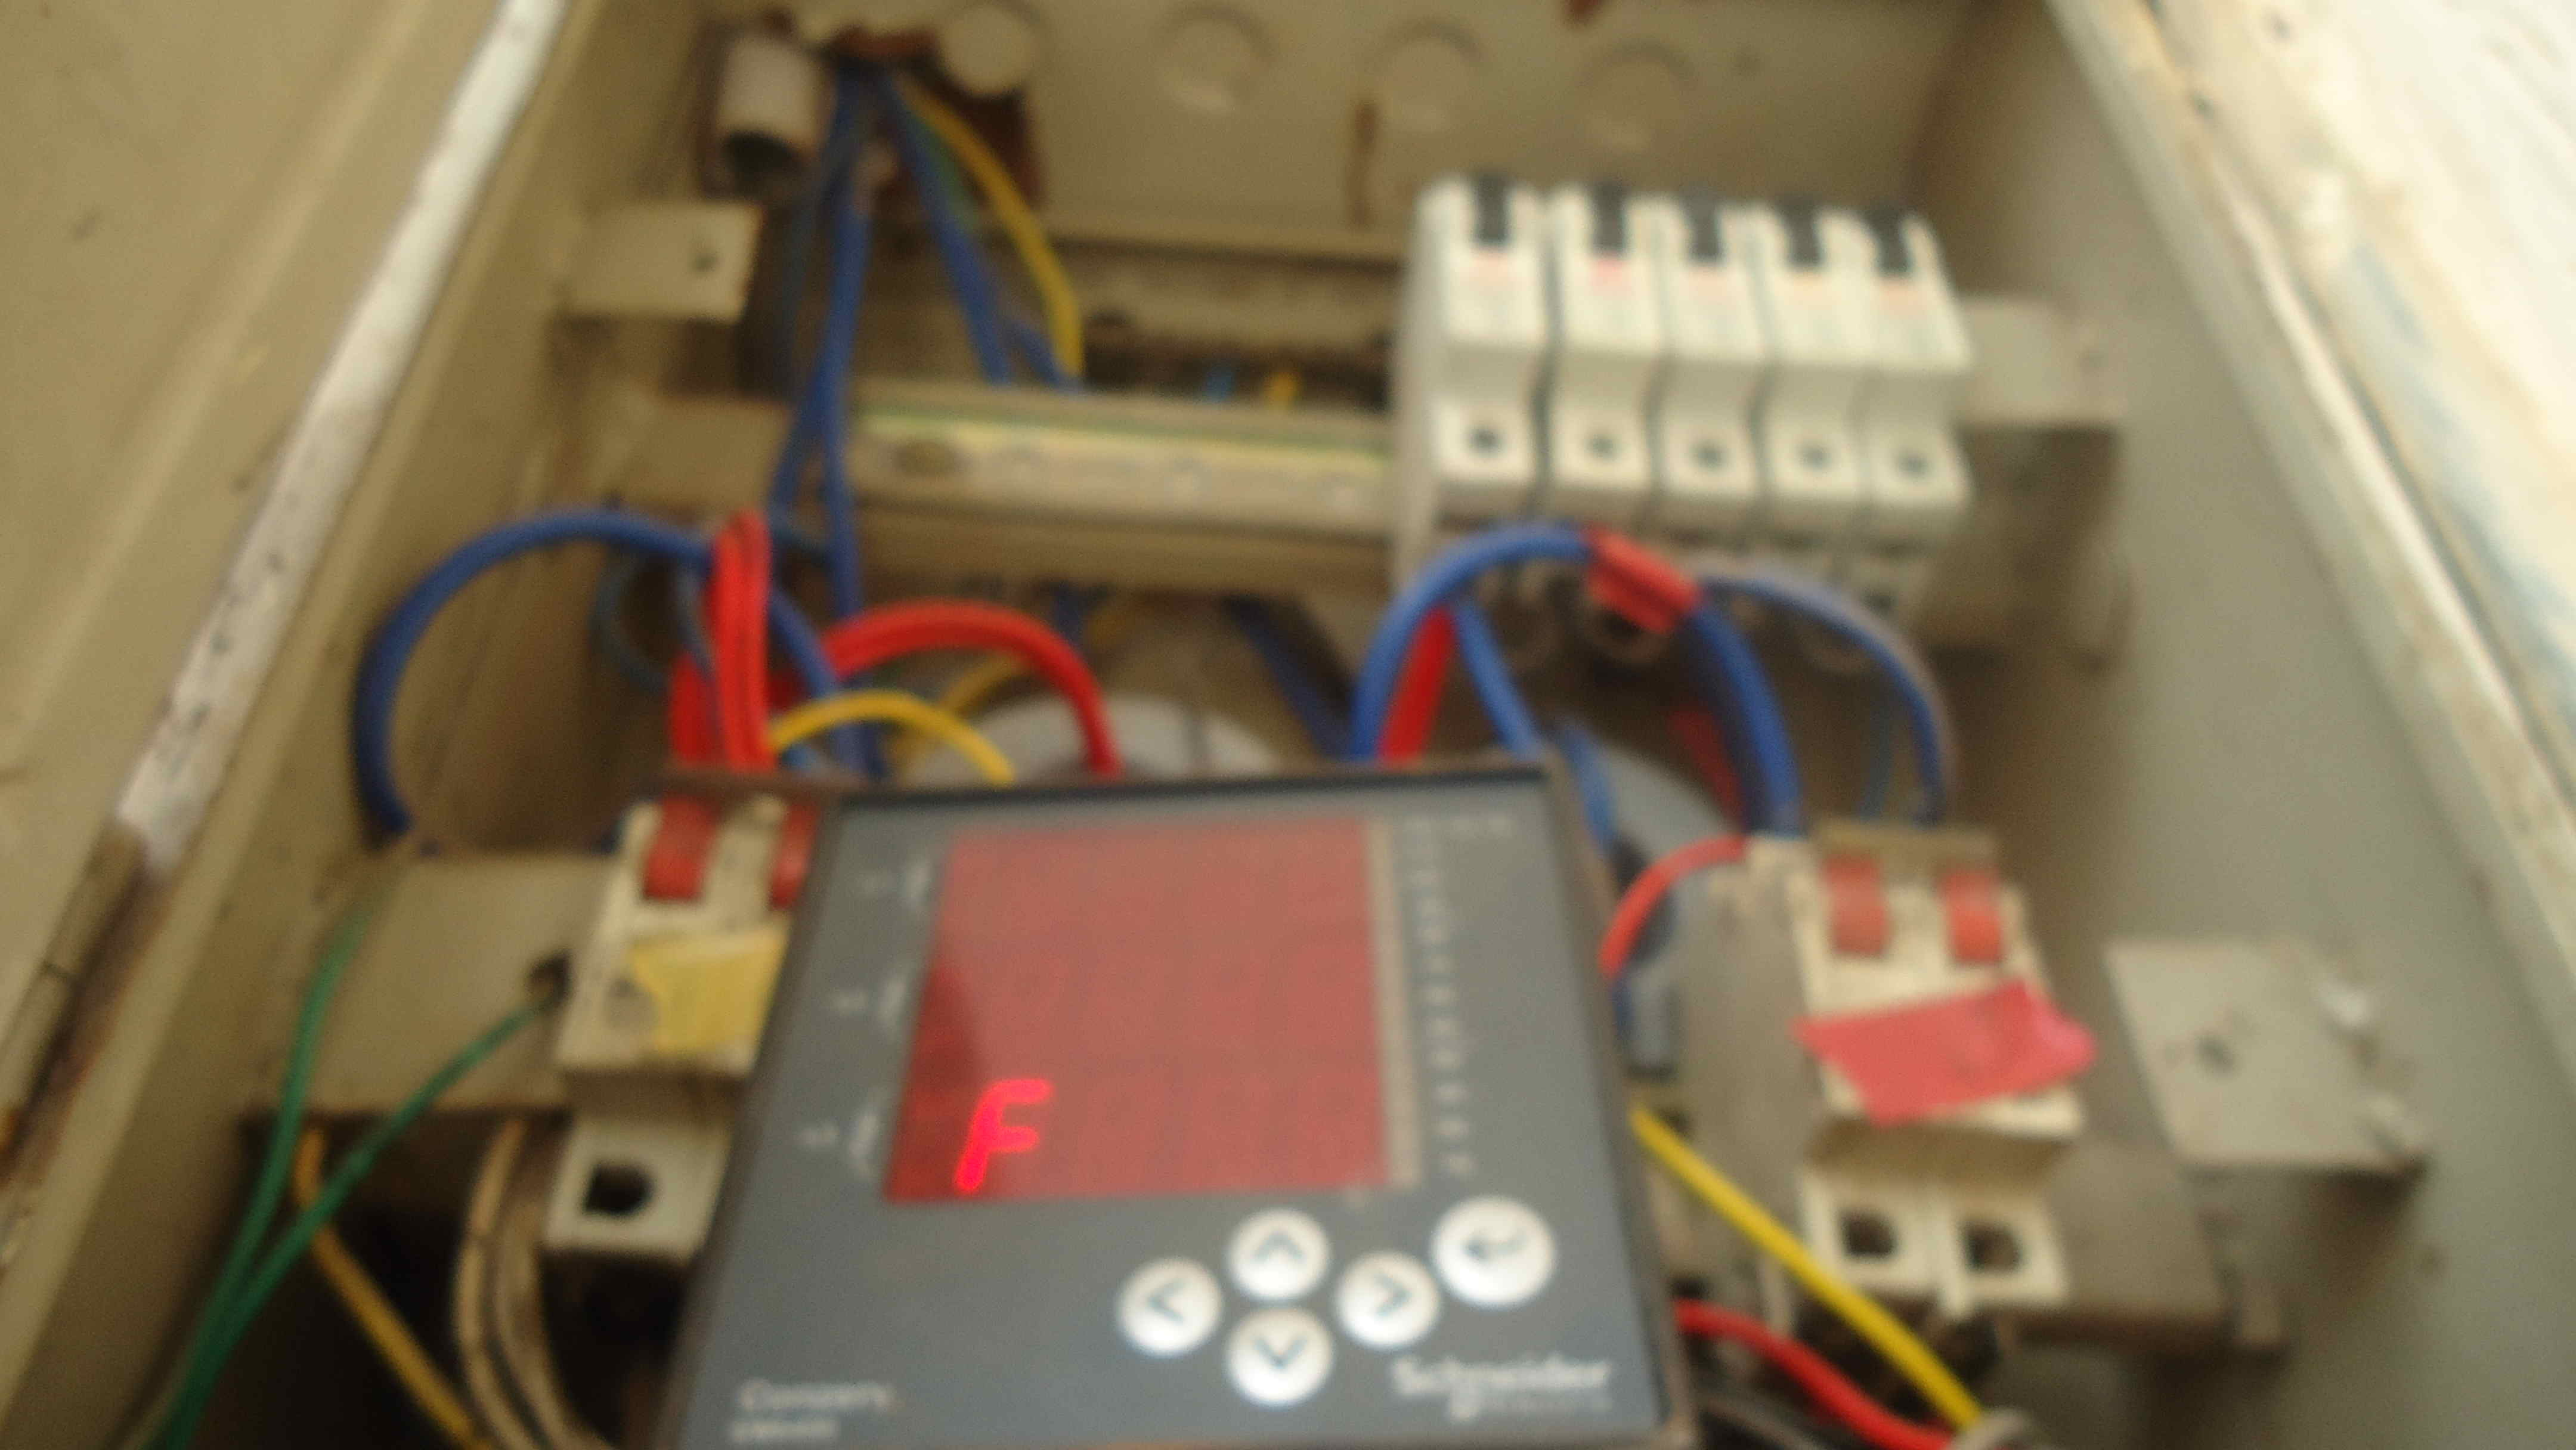
\includegraphics[scale=0.03]{./figures/electric_meter_2.jpg}}
     \subfloat[\scriptsize In house CT monitoring system]{
        \label{fig:ct}
        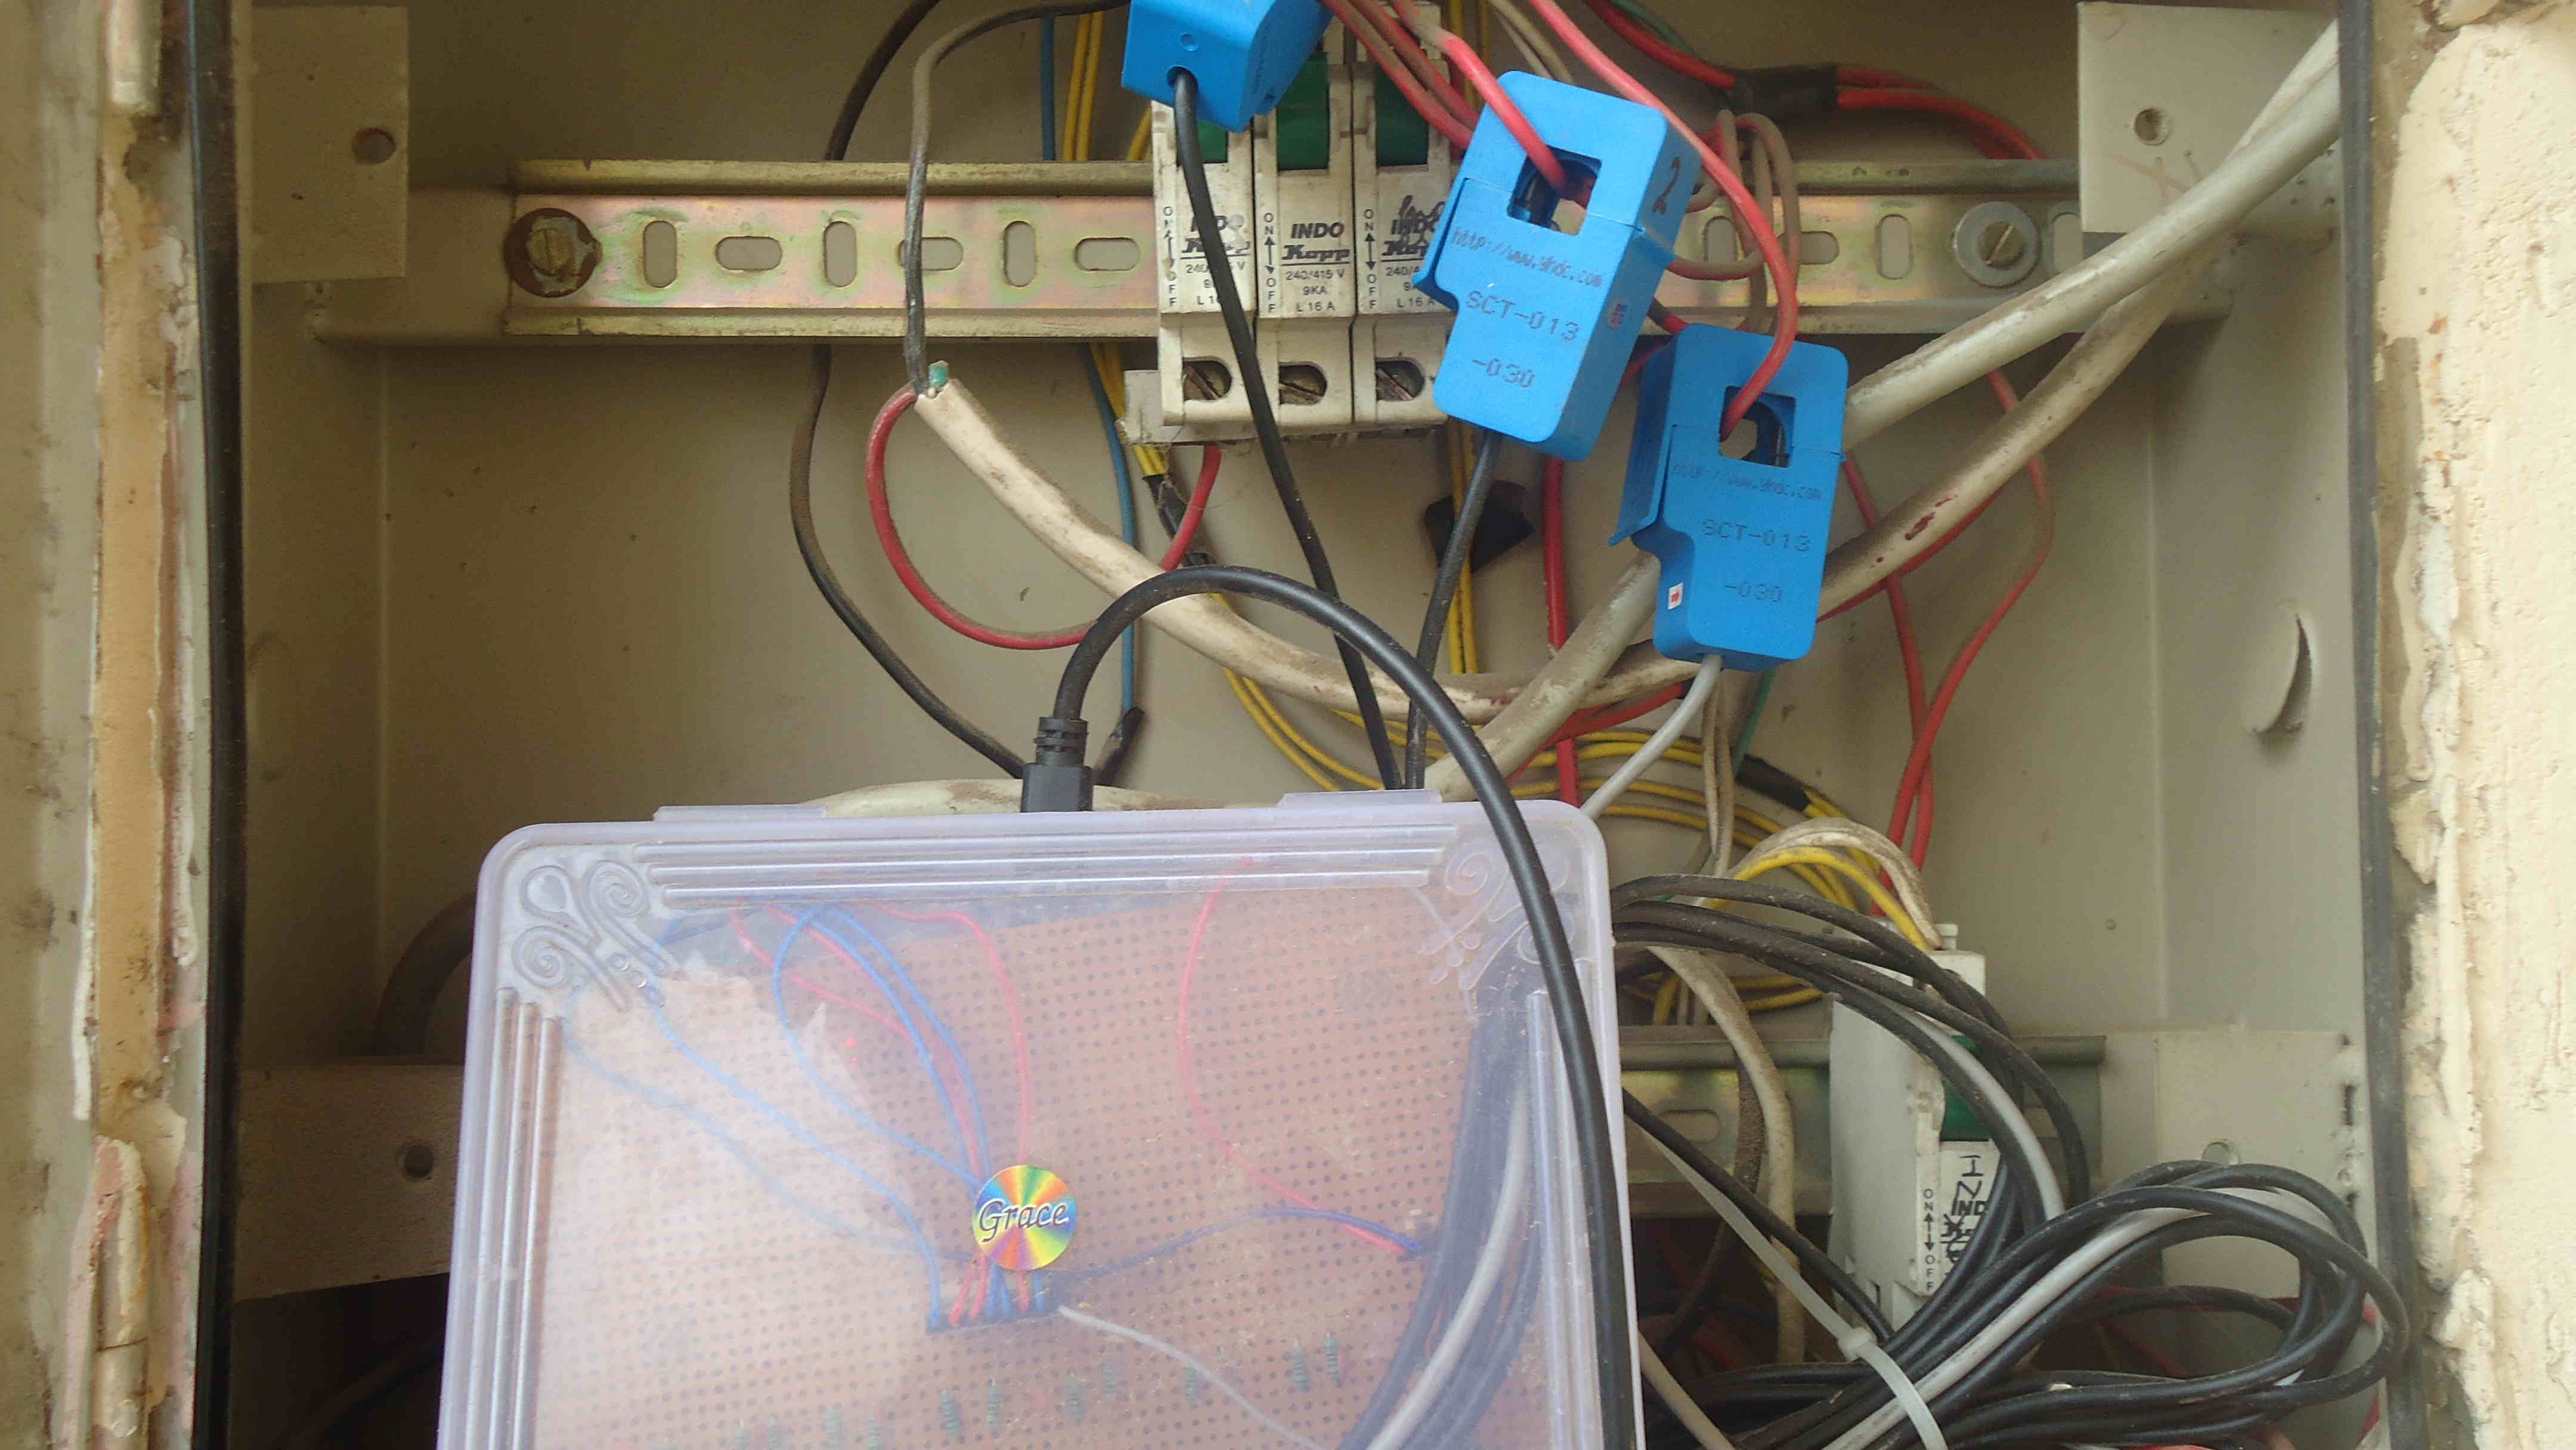
\includegraphics[scale=0.03]{./figures/mcb.jpg}}
     \subfloat[\scriptsize Appliance level monitoring using jPlug]{
             \label{fig:jplug}
             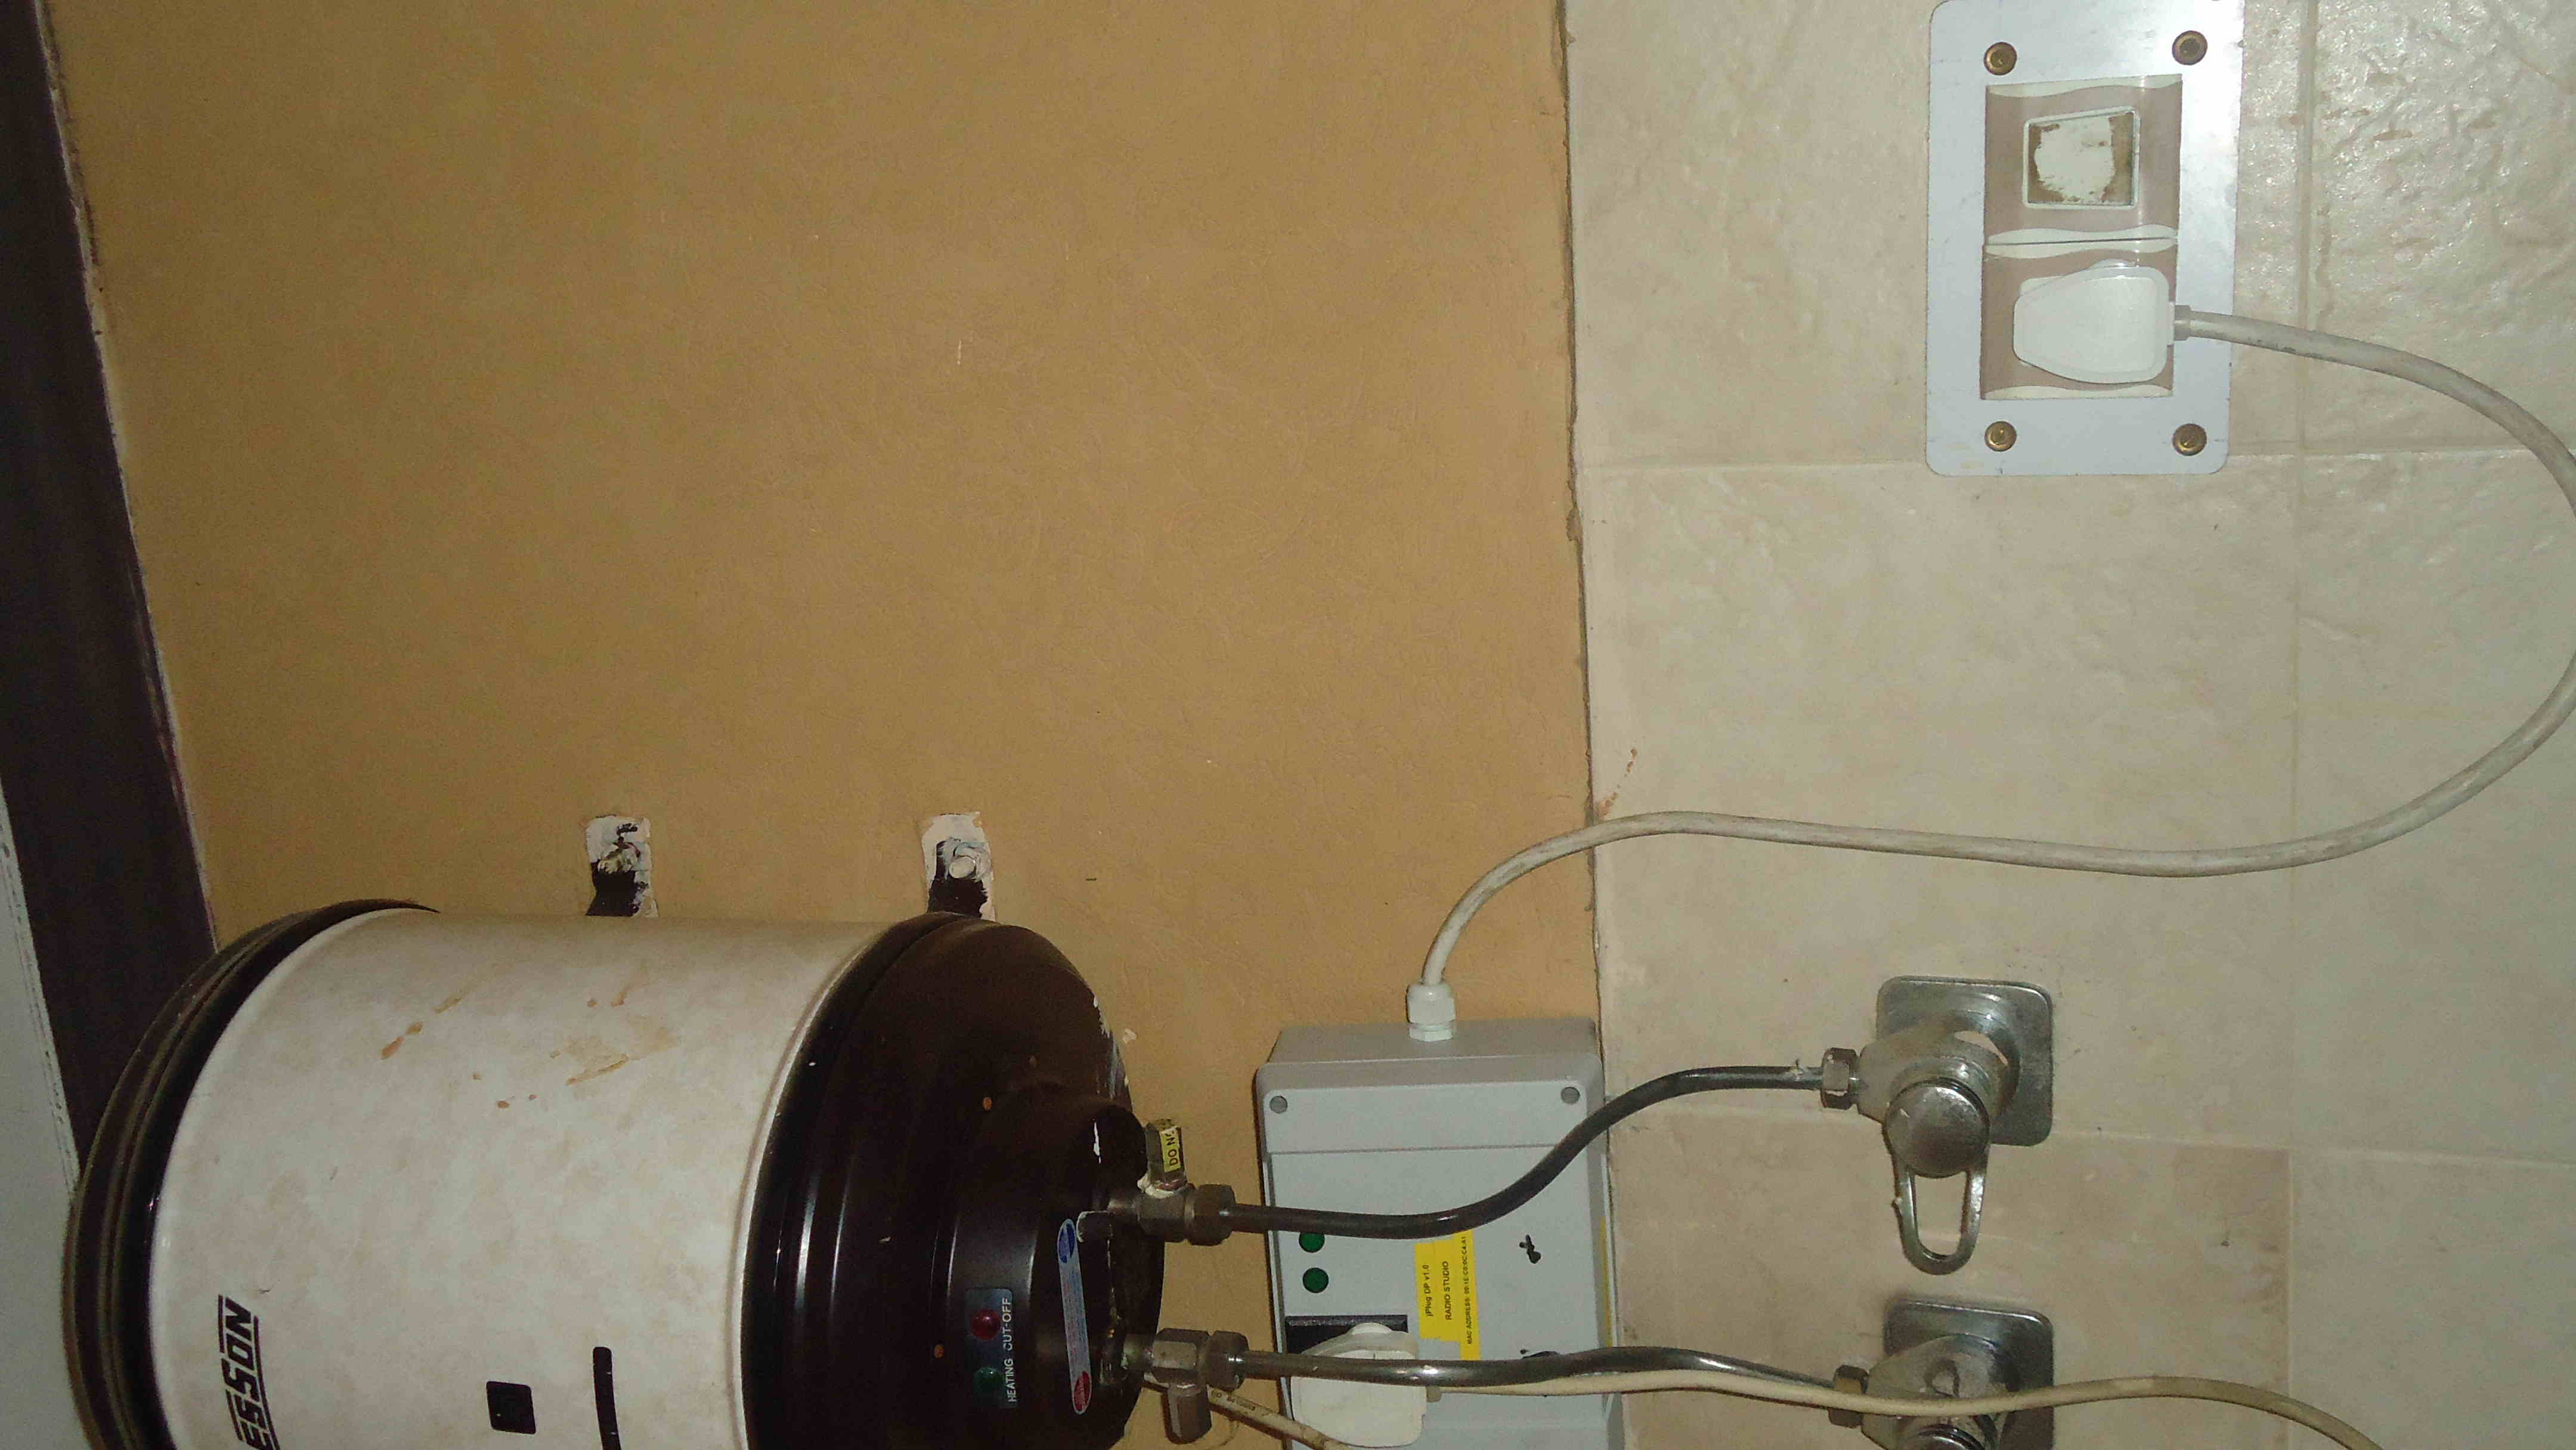
\includegraphics[scale=0.03]{./figures/jplug.JPG}}
          \subfloat[\scriptsize Appliance level monitoring using Current Cost CT]{
                  \label{fig:cc}
                  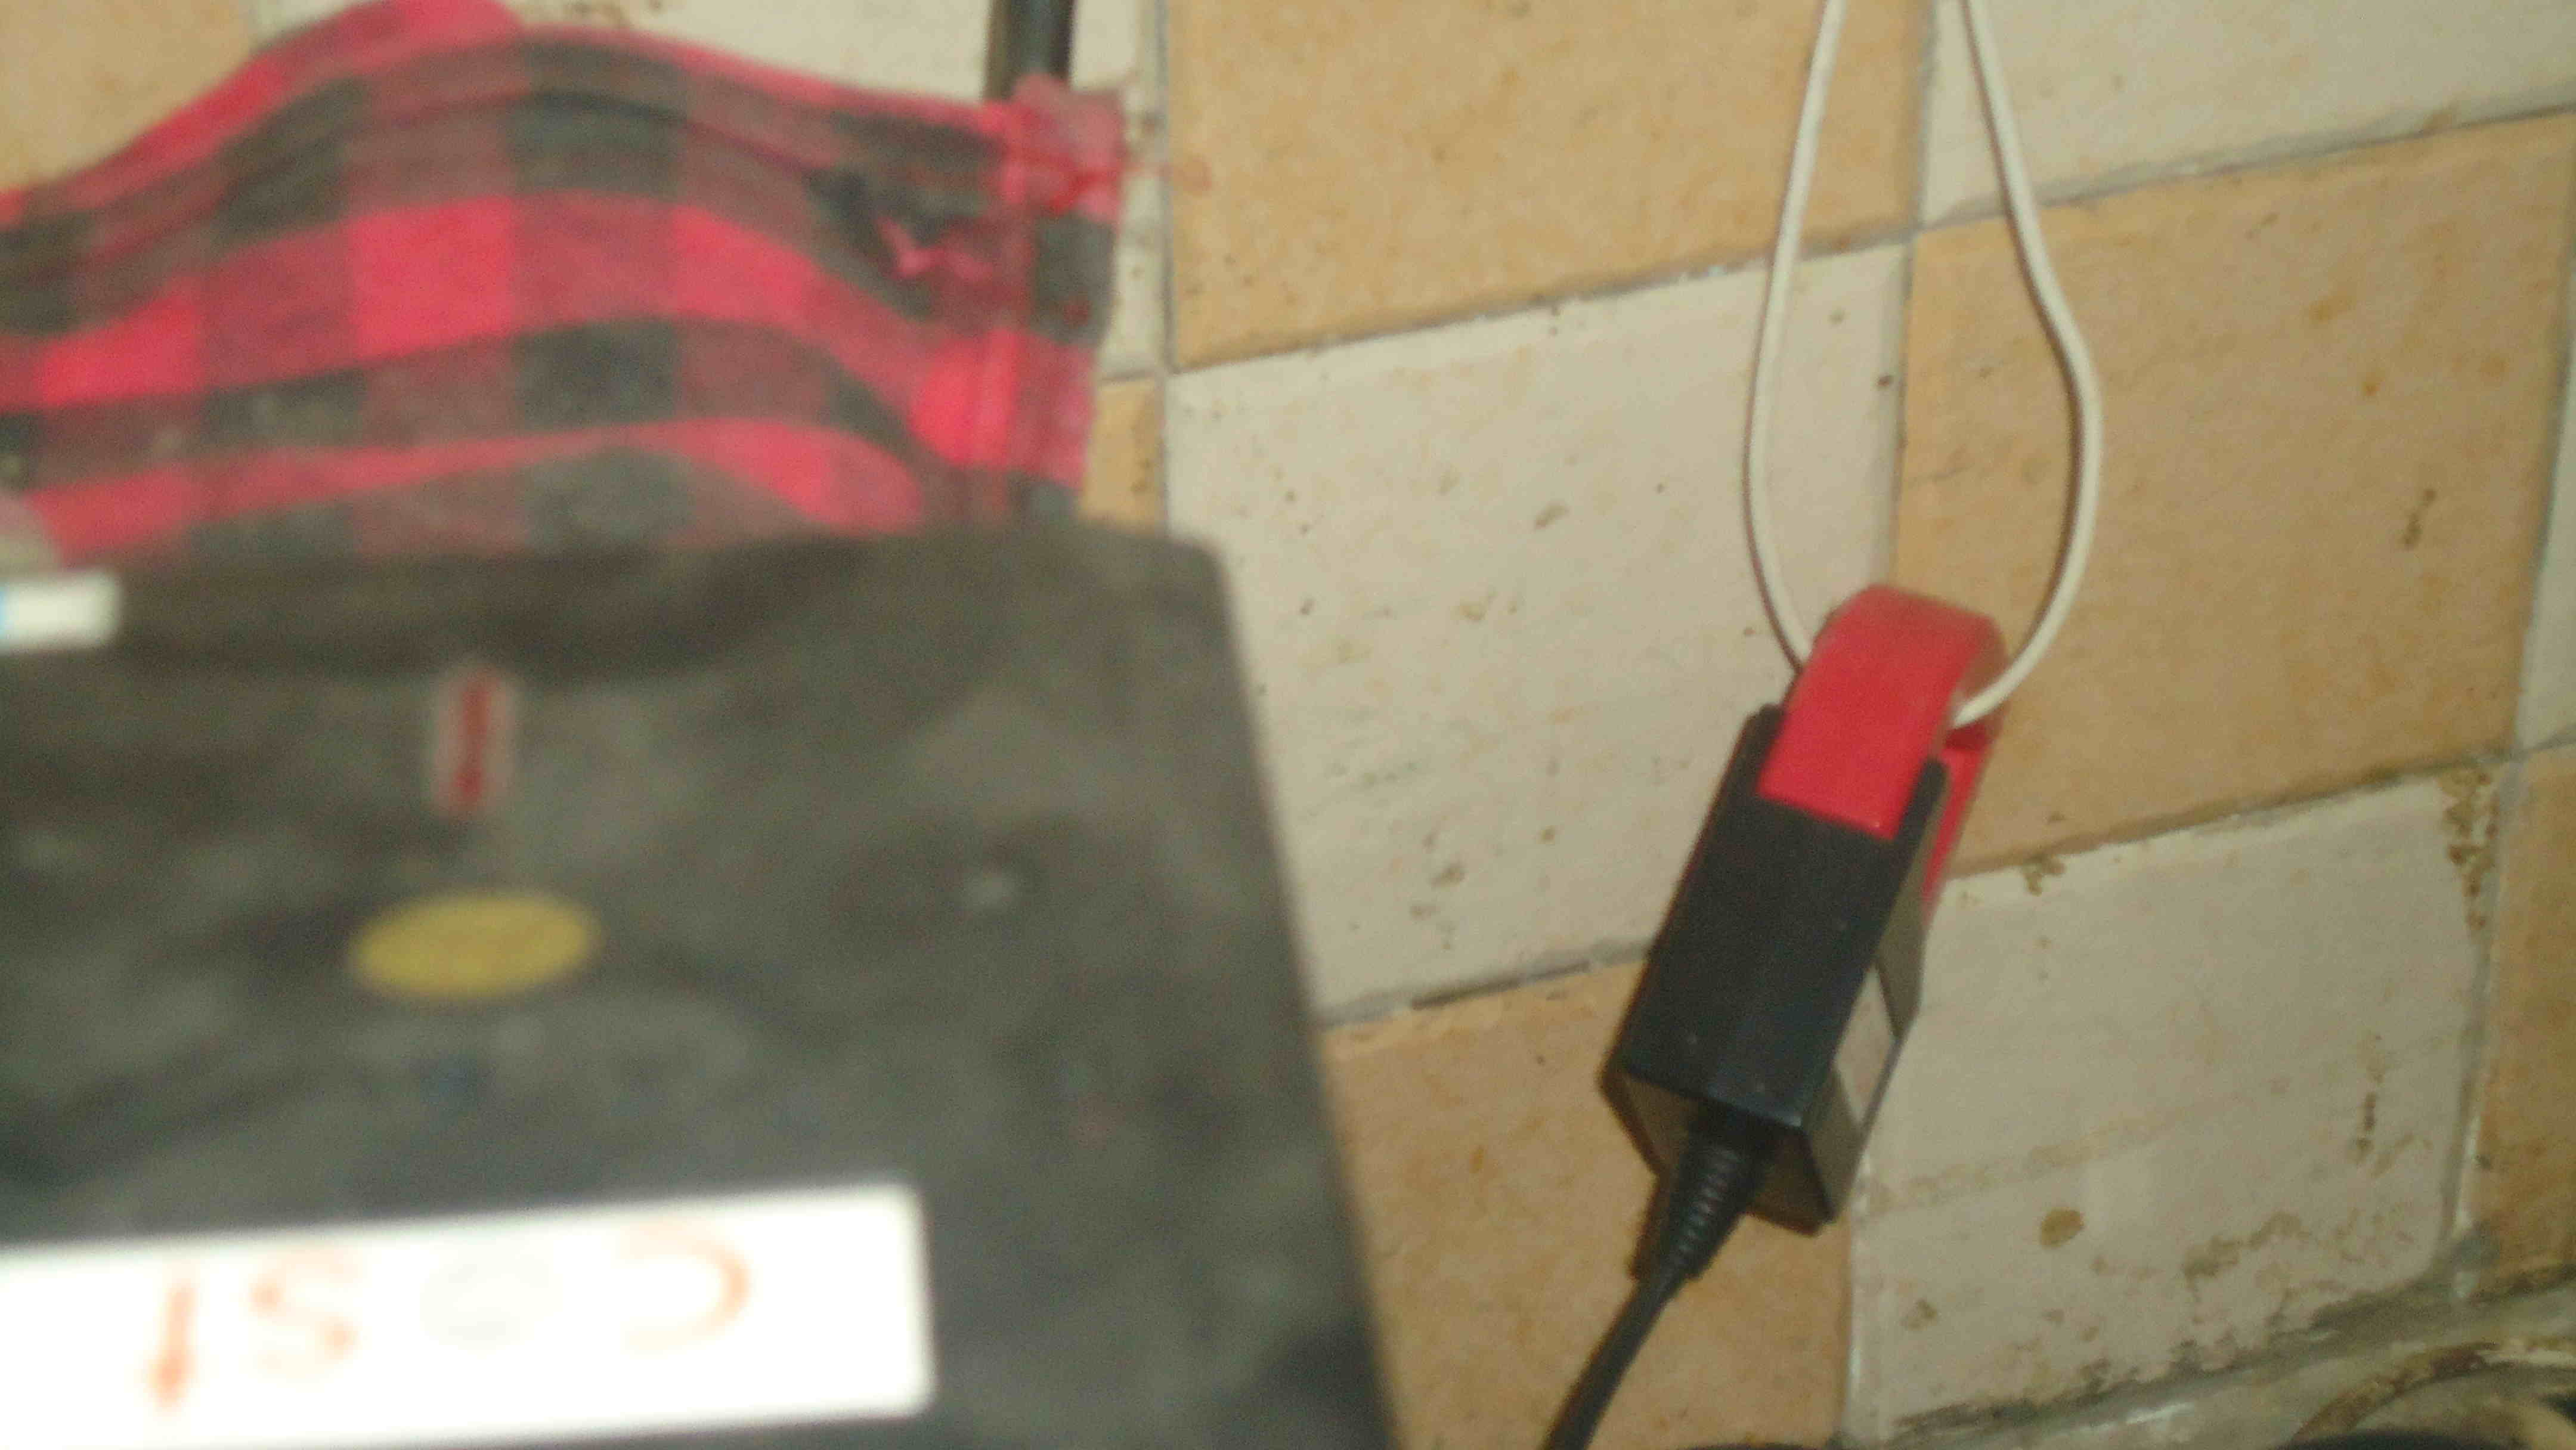
\includegraphics[scale=0.03]{./figures/cc.JPG}}
    %\hspace{0.02\columnwidth}
    \newline
    \subfloat[\scriptsize Water Meter]{
    \label{fig:water_meter}
        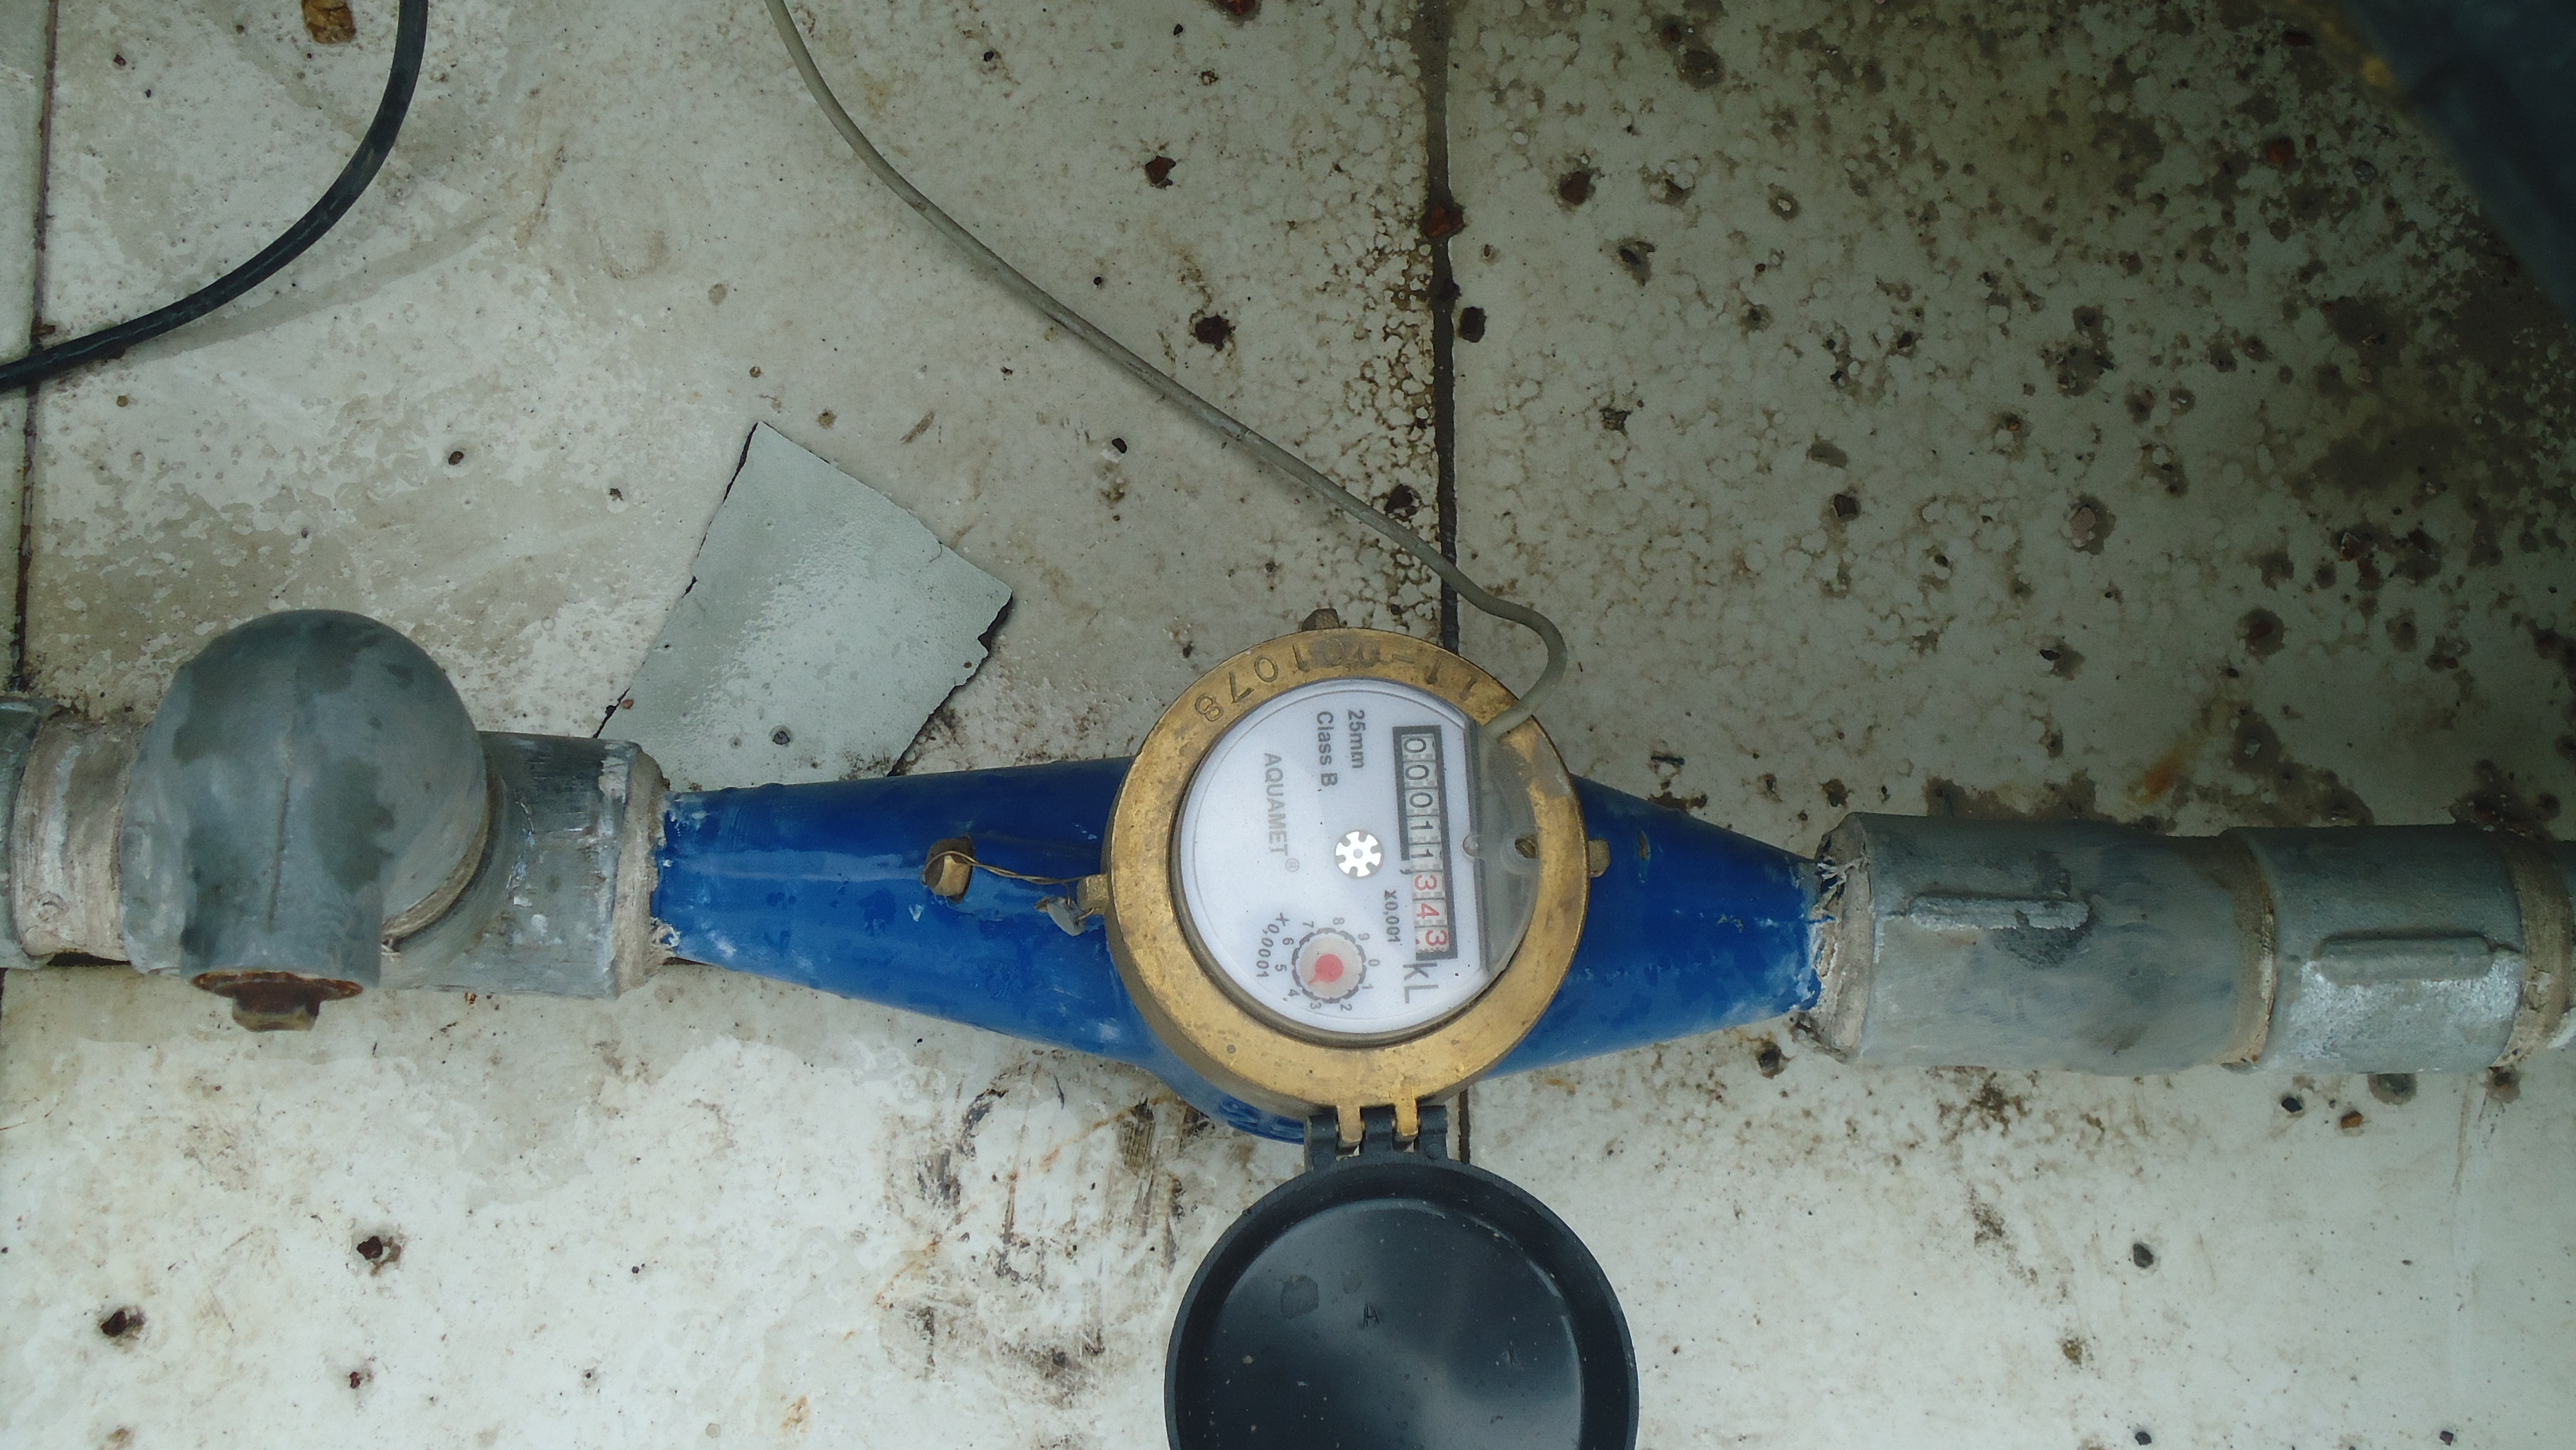
\includegraphics[scale=0.03]{./figures/water_meter.JPG}}
     \subfloat[\scriptsize Android phone and Homeseer Zwave multisensor used to measure ambient parameters]{
        \label{fig:ambient}
            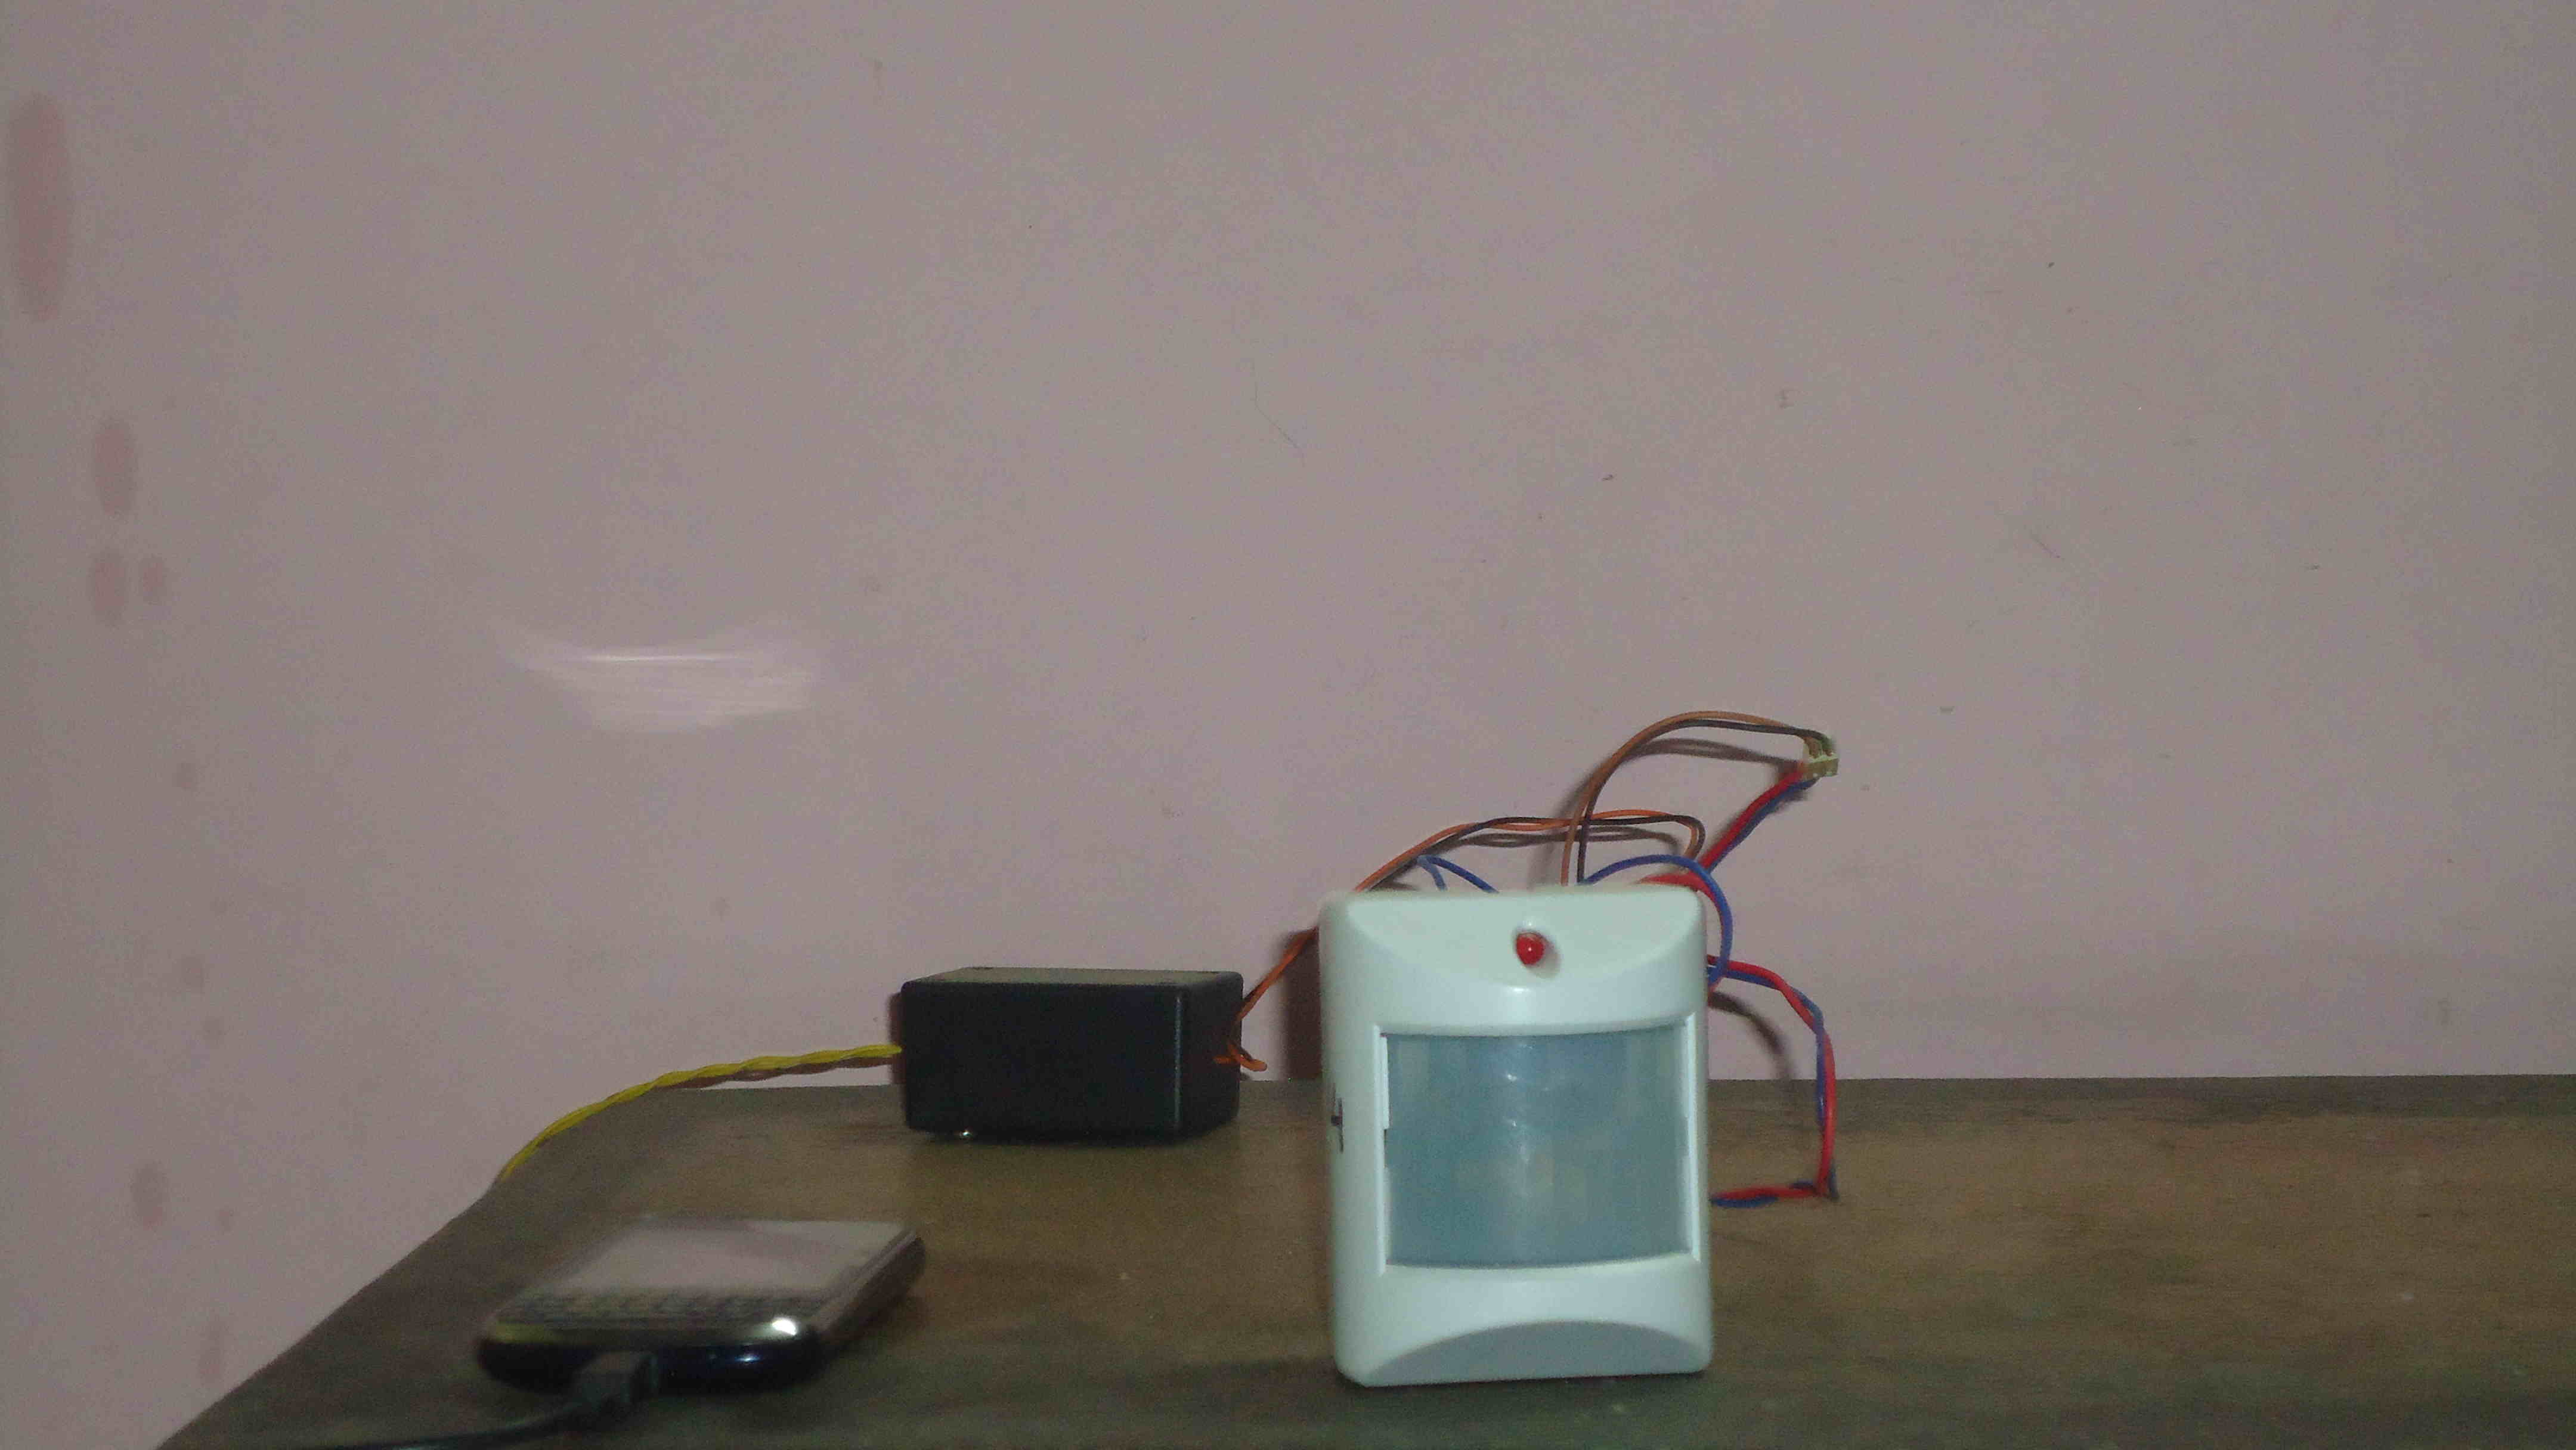
\includegraphics[scale=0.03]{./figures/ambient.JPG}}

    \caption{Deployment Pictures}

    \label{fig:deployment}

\end{figure*}

\section{Learning}
In this section we discuss the learning from previous work in similar domains and present unique aspects which came up in our deployment.
\begin{itemize}

\item Homes are not power panacea. We have a very special case of electricity failure. Add figure
for electricity number of hours failure, failure by n'th hour, hist of failure hours
\item Homes have poor connectivity. This forced us to develop a different paradigm which we call Sense-Store-Transfer. This is shown in \figref{fig:network}

\item Homes are hazardous environments
\begin{itemize}
\item Multi failed when put on inverter point
\item Node in one room will always fail
\item Wire snag and how it led to data loss of node 4
\end{itemize}

\item Homes are remote environments:
We had to raise ~60 new issues on Github. We first did deployment in researchers home which had full access to all nodes.
We also provided alerting mechanisms.

\item User participation
Even at researchers home, had asked the researcher to take notes. But even his engagement was not 100 \%.

\item Aesthetics matter
\begin{itemize}
\item LED in night \figref{fig:led}
\item Noise- Noisy SMPS due to dust. Unique to our setting. Figure from FunF showing sound level before and after cleaning.
\end{itemize}

\item Simplify the architecture
We used Load-Store-Forward. Describe this in more detail and relate to earlier n/w connectivity.
Also when number of systems is so large, simple CSV uploading is the best mechanism.

Wherever possible use Ethernet with repeaters. Also, RPi are known to have problems with WiFi.

\item Importance of meta data and calibration
Figure showing power consumption of ref. after repair
Figure showing different measurements for same appliance
Figure showing voltage fluctuations

\item Provision for more sensors than actual number required. x jplug, y multisensor failed due to ..
\item Non availability of sensors in local markets

\end{itemize}
\begin{figure}     
    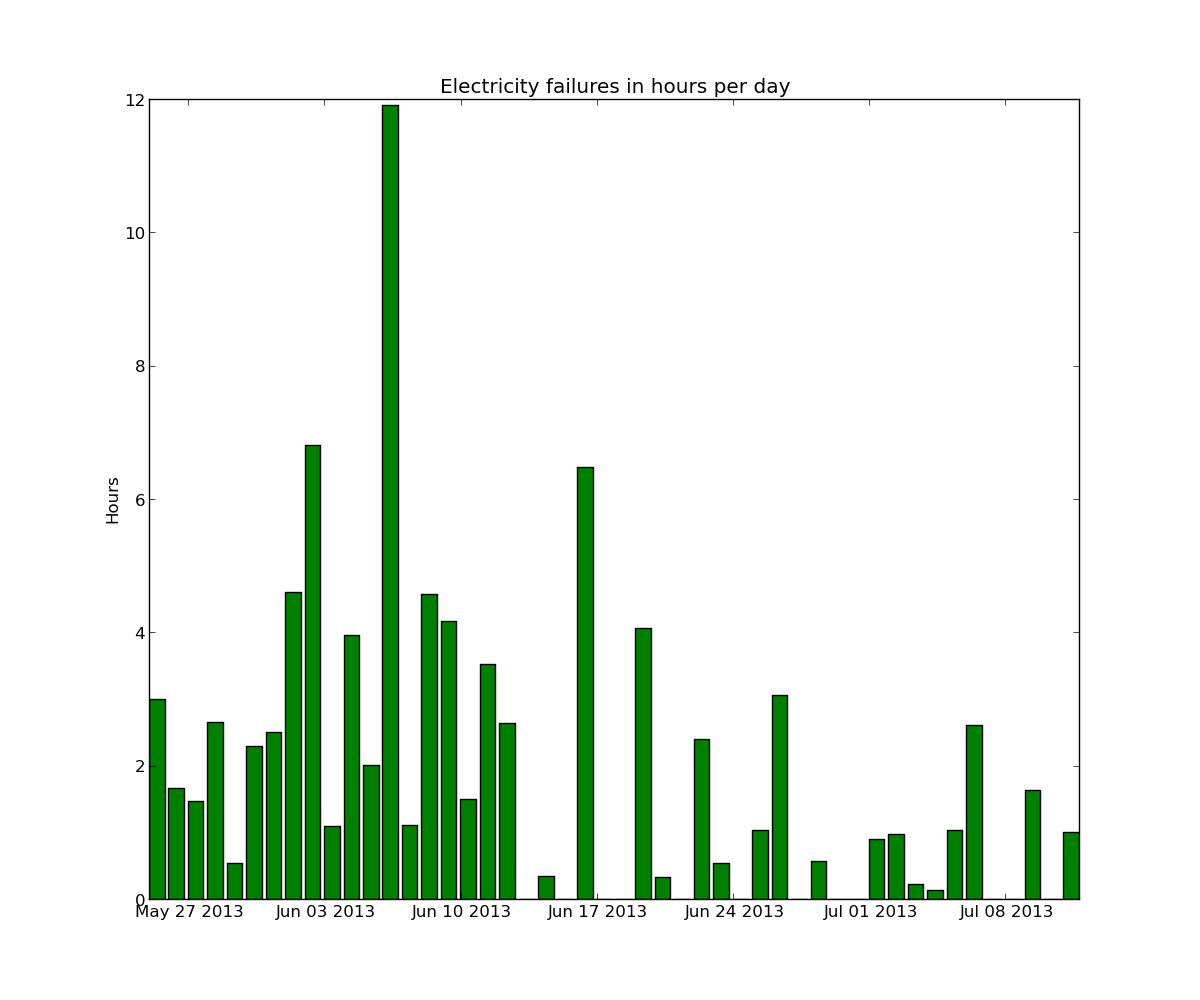
\includegraphics[scale=0.30]{./figures/electricity.png}    
    \caption{Electricity failure in hours}   
    \label{fig:failure_hours}   
\end{figure}

\begin{figure}     
    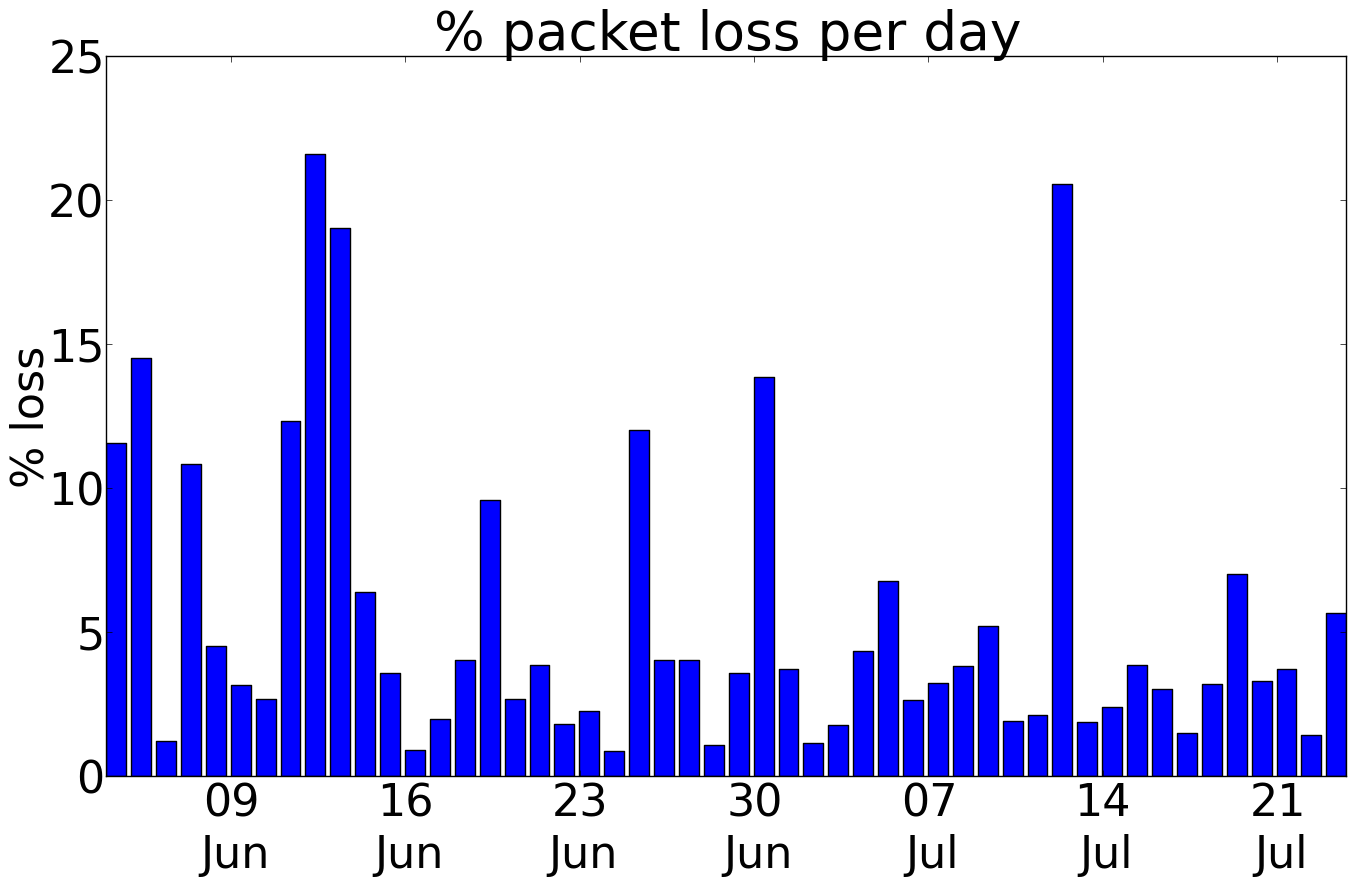
\includegraphics[scale=0.30]{./figures/network.png}    
    \caption{Overall packet drop while accessing internet}   
    \label{fig:network}   
\end{figure}

\begin{figure}     
    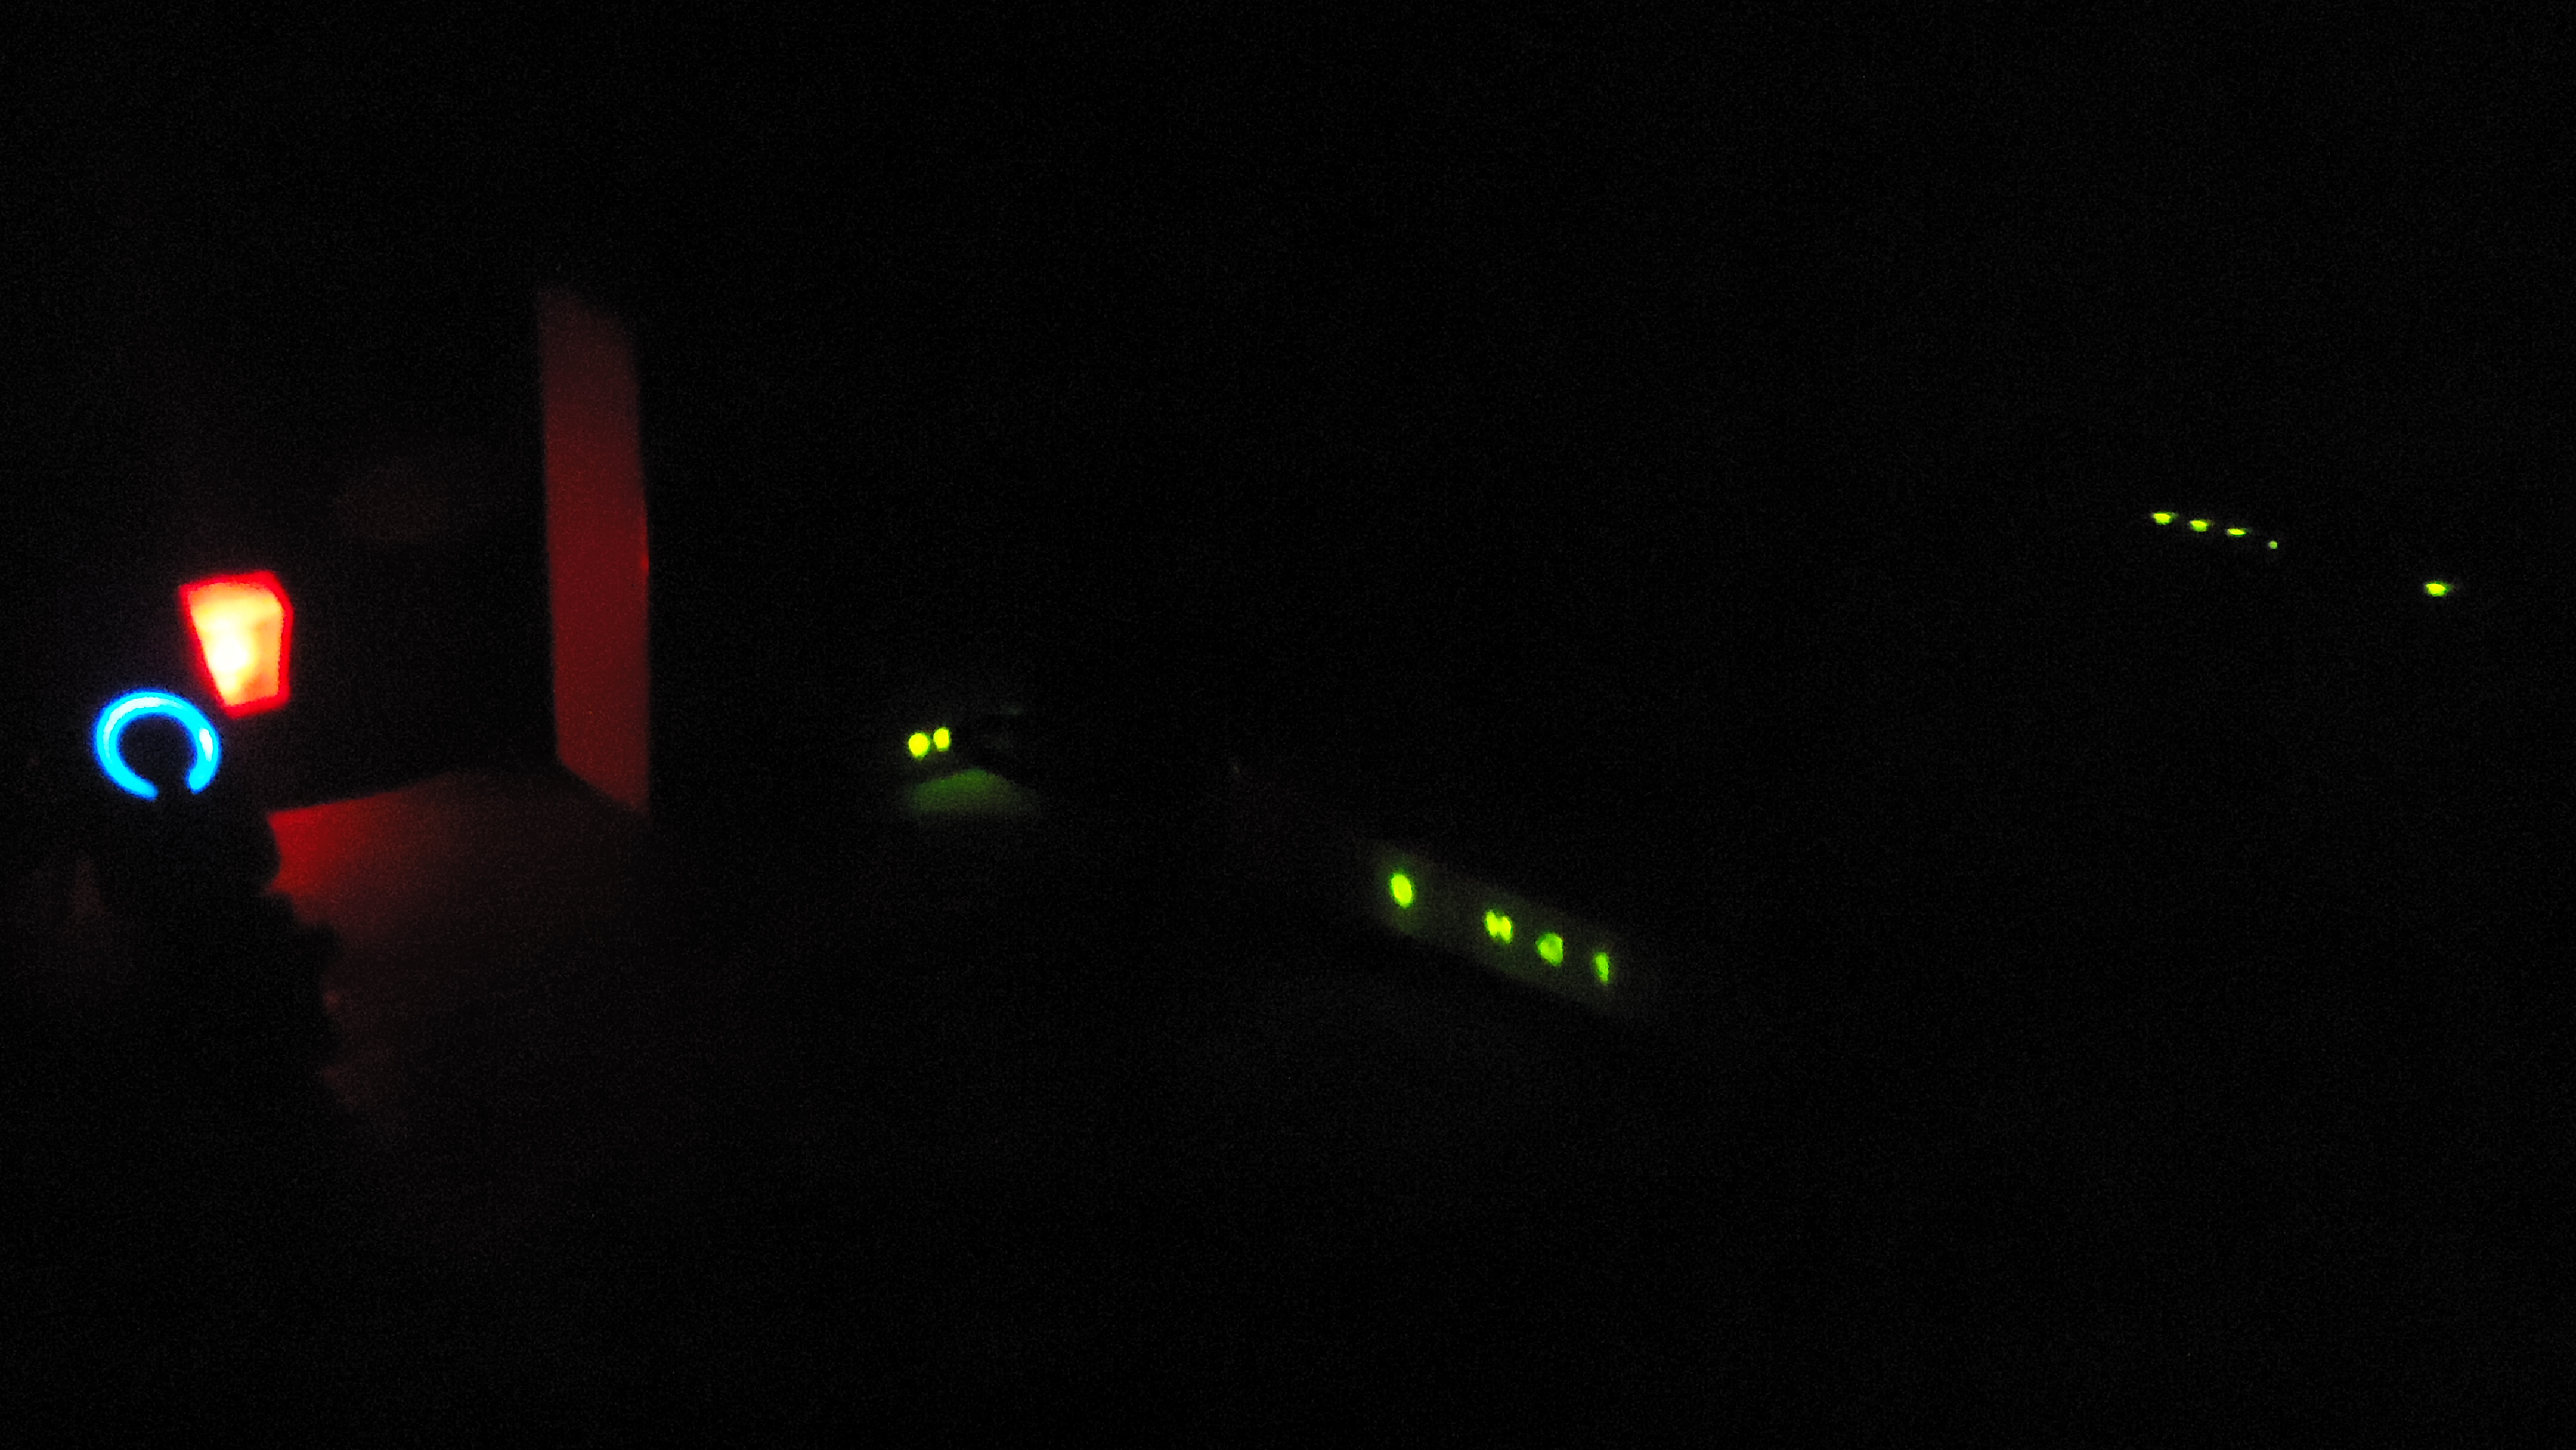
\includegraphics[scale=0.04]{./figures/led.JPG}    
    \caption{LED glowing in the night}   
    \label{fig:led}
   
\end{figure}

\section{Case Studies}
In this section we present some case studies from the data collected in this deployment.
\subsection{Correlating Events and Activity Detection}
In this section we show how multi-modal data can be used for activity recognition. Following plots show the same.


\subsection{Water-Energy Nexus}
\subsubsection{Water Filter}
In this section we find out the effective cost of 1 litre of water. RO is known to waste a lot of water. From the water meter we observe the amount of water consumed to fill 1 litre of water. We also see the corresponding power draw of the RO. Thus, we can see that water has energy embedded in it.

\subsubsection{Electric Motor}
Another unique aspect of our setting is the use of electric motor to pump water. Figure showing 1 litre events before motor was turned on and figure showing 1 litre events after motor is turned on.
Figure showing power consumption incurred by the use of motor.

\subsection{Energy conscious habits}
Figure showing how i turn the AC at 16 degrees and turn it off before going to sleep.

Running the ref. in least cool cooling mode and the impact it has.

\subsection{NILM}
Will be tough to do in timeframe.

To highlight any thing or add new stuff write like this in red

\redcolor{This is my comment. I would also do ... and put this image and put this table and so on and so forth}

\section{Conclusions and Future Work}


\balance
\bibliographystyle{abbrv}
\bibliography{references}  % sigproc.bib is the name of the Bibliography in this case
\end{document}
